\section{L'Allemagne et le BND}

Le BND\footnote{Bundesnachrichtendienst} est le service de
renseignement extérieur allemand, et le pendant technique de la NSA en
Allemagne. Les détails exacts de leur coopération ne sont pas tous connus, mais
on peut au moins citer quelques événements récents qui mettent en lumière des
liens de coopération étroits (bien que moins solides qu'avec le GCHQ).

\subsection{Opération EIKONAL}

Il existe actuellement très peu de détails techniques sur cette
opération, bien que de nombreux documents et témoignages soient venus récemment
(mai 2015) apporter un éclairage nouveau sur ce programme qui s'est déroulé entre 2004 et
2008.\newline

Ces nouveaux éléments ont été apportés par les journaux allemands
Süddeutsche Zeitung\cite{sudde}, NDR et WDR\cite{NDR}, et montrent que la BND,
en partenariat avec Deutsche Telekom, a placé des équipements réseau (des
sondes, en l'occurrence) fournis par la NSA au sein du noeud d'échange (noeud
PoP) maintenu par l'opérateur allemand, à Francfort.

\vspace{0.7cm}
\begin{figure}[h]
\centerline{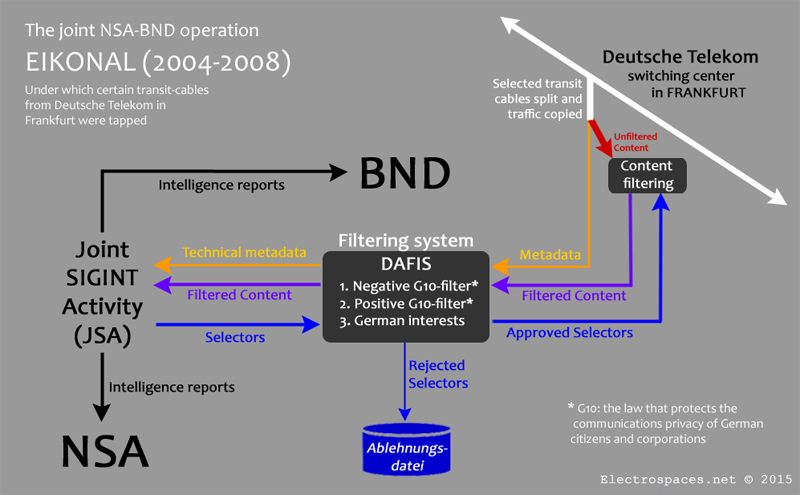
\includegraphics[width=11cm]{eikonal1.jpg}}
\caption[Architecture de l'opération EIKONAL]{Architecture
technique de l'opération}
\label{fig:eikonal1}
\end{figure}

Ce schéma montre l'organisation technique de l'opération : les
méta-données ainsi qu'une partie spécifique du trafic sont récupérées et passent
à travers un filtre nommé DAFIS\label{dafis}, qui sert à différencier les
communications provenant de citoyens allemands (que la BND n'a pas, légalement, le droit
d'espionner, de part son statut de service de renseignement \emph{extérieur}.
Dans ce cas de figure, elle doit passer par un <<~ordre G10~>> pour accéder
aux communications).
En fonction des résultats après passage dans le filtre, les données sont soit
renvoyés à la BND, soit directement à la NSA. Le schéma décisionnel est
reproduit ci-dessous :

\begin{figure}
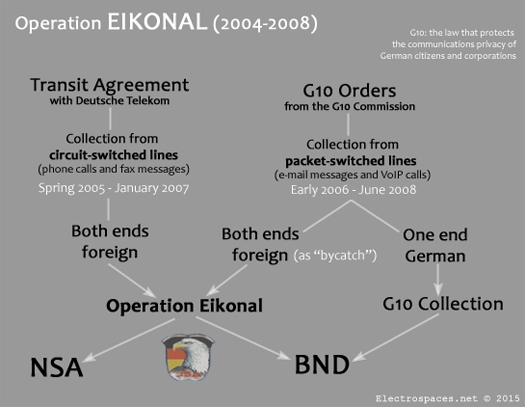
\includegraphics{eikonal2.jpg}
\caption[Schéma décisionnel de l'opération EIKONAL][6pt]{Schéma décisionnel}
\label{fig:eikonal2}
\end{figure}

La mise sur écoute concernait plus spécifiquement le câble FFM 21
reliant le Luxembourg et Francfort, contenant des canaux de fibres optiques
reliant le Luxembourg à Moscou, Prague, Vienne (où se trouvent des instances de
l'ONU) et Ankara\citep{eikonal3}. Cela permettait à la NSA d'accéder à une
partie du monde auquel elle est très mal reliée directement.

\begin{figure}[!h]
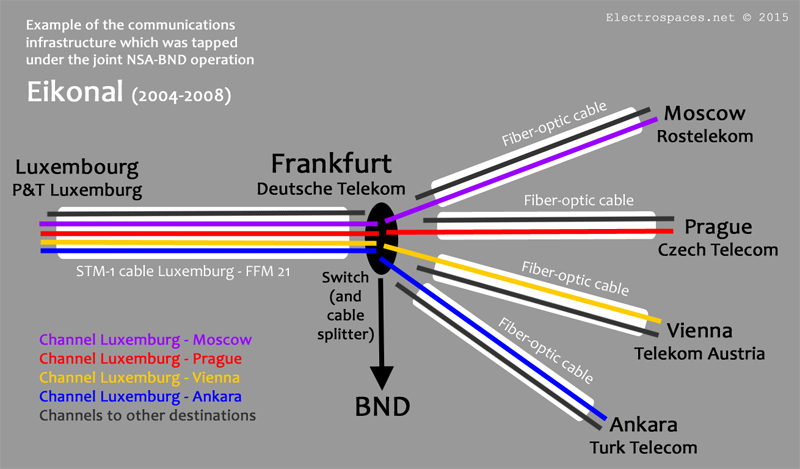
\includegraphics{eikonal3.jpg}
\caption[Schéma des canaux mis sur écoute][6pt]{Schéma des canaux mis sur
écoute}
\label{fig:eikonal3}
\end{figure}

\newpage
EIKONAL a fait parti d'un programme plus large de la NSA de
coopération avec des pays dits <<~tiers~>>, qui sont des pays ne faisant pas
partie de Five Eyes, mais qui coopèrent avec la NSA, de façon ponctuelle (comme
ici) ou de façon plus constante. Ce programme est nommé RAMPART-A, et concerne
un nombre inconnu de pays. L'Allemagne est connue pour en faire partie, alors
que de forts soupçons pèsent sur le Danemark\cite{danemark} et qu'il est
rapporté, via des slides publiées par Snowden, qu'au moins cinq pays possèdent
des moyens similaires déployés sur leurs réseaux nationaux.

\begin{figure}
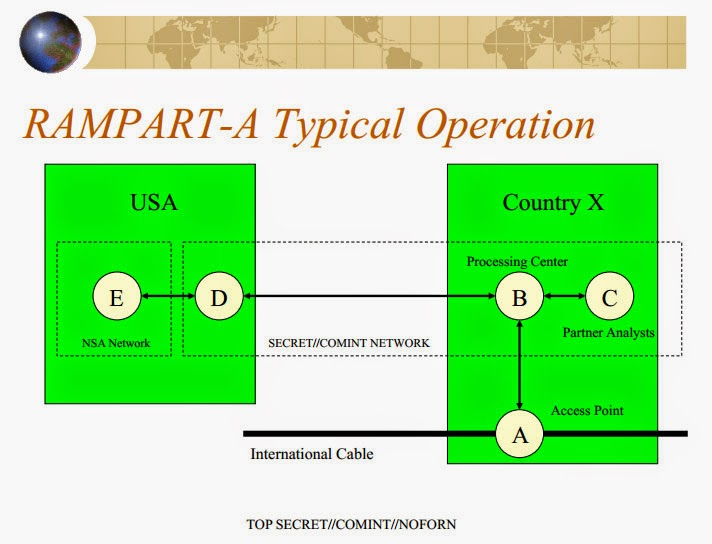
\includegraphics{rampart.jpg}
\caption[Schéma de l'opération RAMPART-A][6pt]{Schéma de l'opération RAMPART-A}
\label{fig:rampart}
\end{figure}


\newpage
\subsection{La station de Bad Aibling : nom de code GARLICK}

\begin{figure}
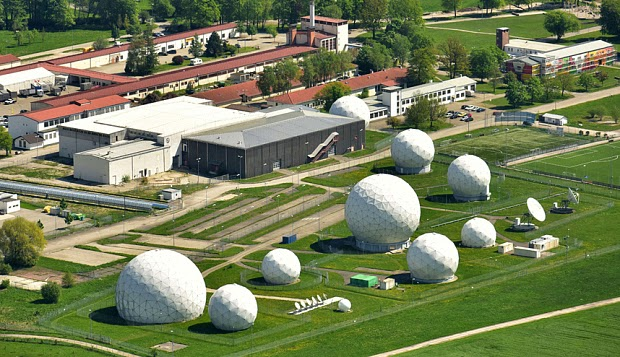
\includegraphics{ba1.jpg}
\caption[Station d'interception de Bad Aibling][6pt]{Station d'interception de
Bad Aibling, opérée par la BND à partir de 2004.}
\label{fig:ba1}
\end{figure}

Cette station est une ancienne station d'écoute du réseau ECHELON,
et appartenait anciennement à la NSA, qui l'a depuis rendue à l'Etat Fédéral en
2004 (tout en gardant une équipe opérationnelle sur le site).\cite{spiegel}

Il fut révélé que la NSA pouvait accéder directement aux données
des interceptions, et fournissait même quatre des cinq listes de sélecteurs
utilisées pour savoir quoi chercher dans le flux de données (adresses IP,
numéros de téléphone, etc). 

Initialement très petites, ces listes ce sont graduellement
remplies, au point que des contrôles manuels ne furent plus possibles. Elles
furent donc envoyées automatiquement plusieurs fois par semaine au siège de la
BND, où elles passaient à travers le DAFIS (voir page \pageref{dafis}) afin
d'exclure les communications impliquant des ressortissants ou citoyens
allemands, puis souvent renvoyées tel quel à la NSA.

Ces sélecteurs furent à l'origine d'un scandale à portée européenne
lorsqu'il fut révélé par certains médias allemands que ces listes contenaient
des entrées visant des employés du groupe Airbus\cite{airbus}.

Au total, la collecte de méta-données, transmises directement à la
NSA après être passées par DAFIS, était de l'ordre de 200-220 millions par jour,
soit environ 6.6 milliards de méta-données collectées par mois\ldots\cite{meta}


\begin{figure}
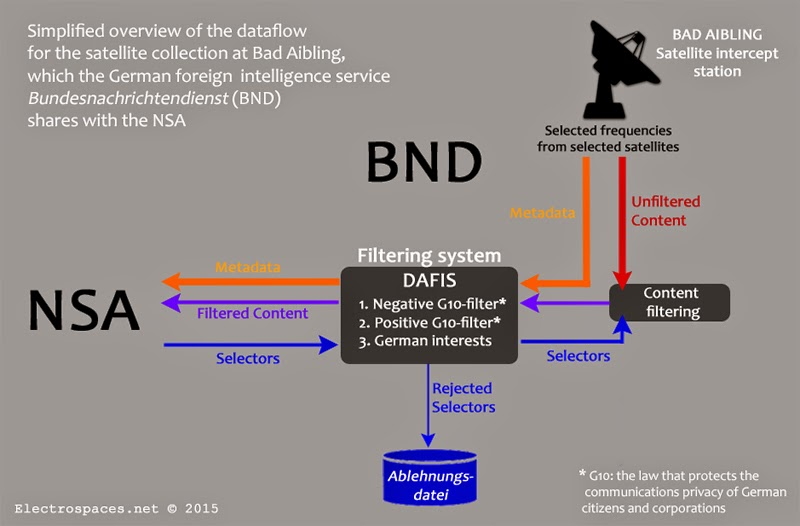
\includegraphics{ba2.jpg}
\caption[Schéma des interceptions à Bad Aibling][6pt]{Schéma des interceptions à Bad Aibling}
\label{fig:ba2}
\end{figure}


\begin{figure}
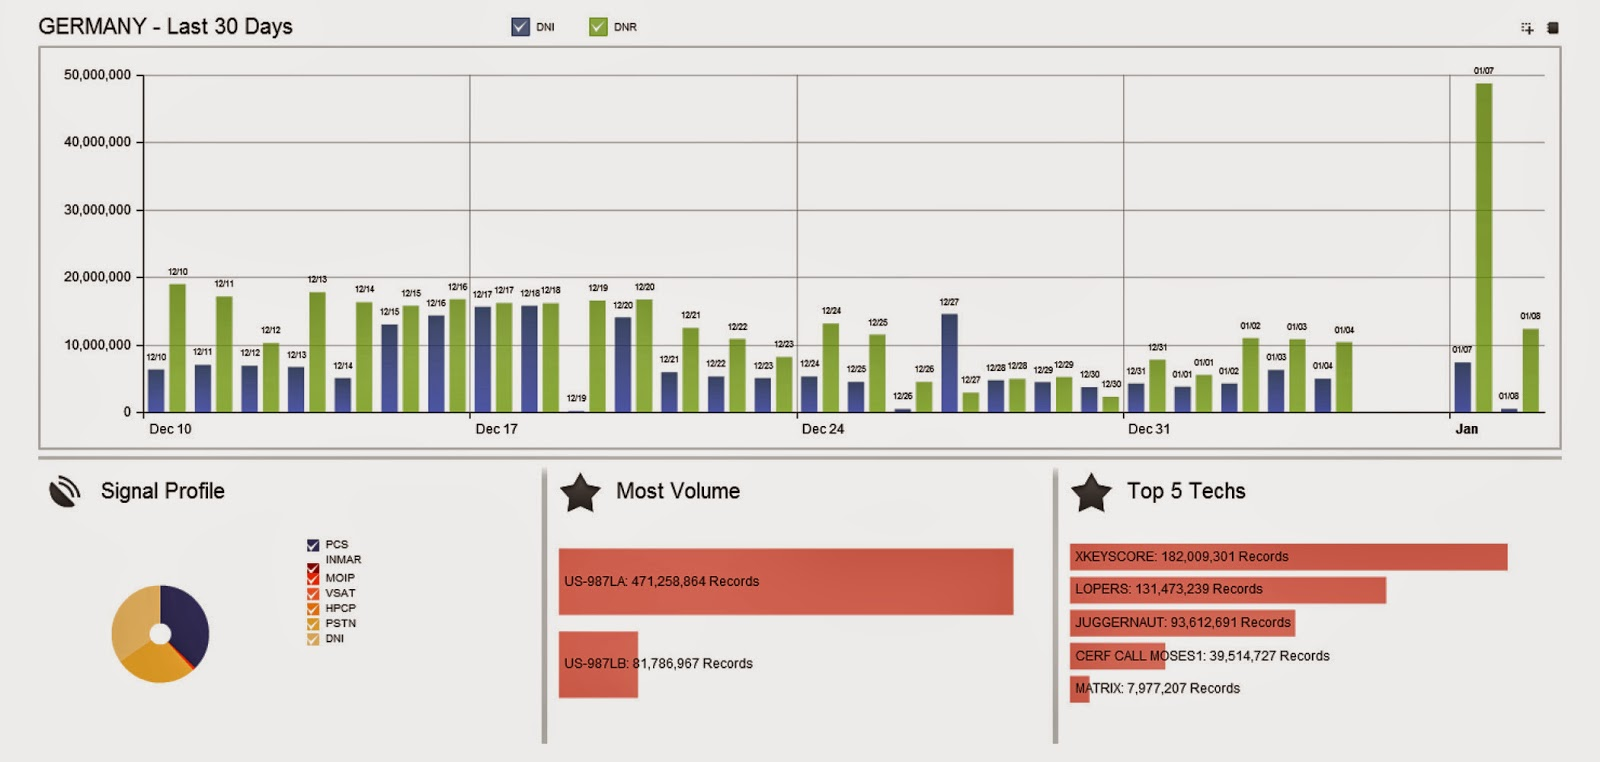
\includegraphics{ba3.jpg}
\caption[Capture écran de BOUNDLESSINFORMANT pour l'Allemagne][6pt]{552 millions
de meta-données entre décembre 2013 et janvier 2013\ldots}
\label{fig:ba3}
\end{figure}